\documentclass{scrartcl}

\usepackage[colorlinks = true, urlcolor = blue, citecolor = blue, linkcolor = red]{hyperref}
\usepackage{listings}
\usepackage{tikz}
\usepackage{xspace}
\usepackage[T1]{fontenc}
\usepackage[scaled = 0.85]{beramono}

\usetikzlibrary{fit}
\usetikzlibrary{positioning}

\lstset{basicstyle = \footnotesize\ttfamily, keywordstyle = \bfseries, breaklines = true, captionpos = b}

\tikzstyle{module} = [draw, very thick, rounded corners]
\tikzstyle{plugin} = [draw, semithick, rounded corners]
\tikzstyle{data} = [draw, semithick, densely dashed, rounded corners]
\tikzstyle{flow} = [draw, semithick, -latex]

\newcommand{\ie}{i.e.\xspace}
\newcommand{\eg}{e.g.\xspace}

\title{CyberTop v1.0 manual}
\author{Politecnico di Torino}
\date{}

\begin{document}

\maketitle

\tableofcontents

\section*{Forewords}

CyberTop (CYBERsecurity TOPologies) is the tool in charge of creating a set of countermeasures against an attack in the SHIELD framework.

This document is split into two pars: the \emph{user manual} is useful to who wants to use the application, while the \emph{developer manual} is useful if you want to extend it. Before delving deep into them, it is a good idea to read the introduction (Section~\ref{sec:introduction}), since it explains several fundamental concepts.

\cleardoublepage
\section{Introduction}
\label{sec:introduction}

The basic work-flow behind CyberTop is illustrated in Figure~\ref{fig:workFlow}.

\begin{figure}[ht]
	\centering
	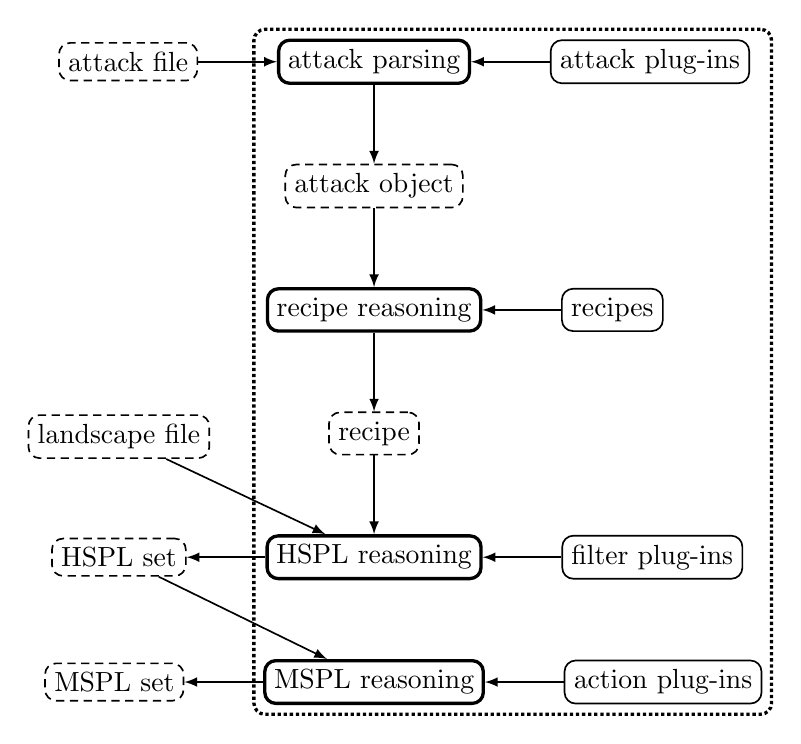
\begin{tikzpicture}
	\node[data] (attackFile) {attack file};
	\node[module, right = of attackFile] (attackParser) {attack parsing};
	\node[plugin, right = of attackParser] (attackPlugins) {attack plug-ins};
	\node[data, below = of attackParser] (attackObject) {attack object};
	\node[module, below = of attackObject] (recipeReasoner) {recipe reasoning};
	\node[plugin, right = of recipeReasoner] (recipes) {recipes};
	\node[data, below = of recipeReasoner] (recipe) {recipe};
	\node[module, below = of recipe] (hsplReasoner) {HSPL reasoning};
	\node[plugin, right = of hsplReasoner] (filters) {filter plug-ins};
	\node[data, left = of hsplReasoner] (hsplSet) {HSPL set};
	\node[data, above = of hsplSet] (landscapeFile) {landscape file};
	\node[module, below = of hsplReasoner] (msplReasoner) {MSPL reasoning};
	\node[plugin, right = of msplReasoner] (actions) {action plug-ins};
	\node[data, left = of msplReasoner] (msplSet) {MSPL set};
	
	\node[draw, densely dotted, very thick, rounded corners, fit = (attackParser) (attackPlugins) (attackObject) (recipeReasoner) (recipes) (recipe) (hsplReasoner) (filters) (msplReasoner) (actions)] {};
	
	\path[flow] (attackFile) -- (attackParser);
	\path[flow] (attackPlugins) -- (attackParser);
	\path[flow] (attackParser) -- (attackObject);
	\path[flow] (attackObject) -- (recipeReasoner);
	\path[flow] (recipes) -- (recipeReasoner);
	\path[flow] (recipeReasoner) -- (recipe);
	\path[flow] (recipe) -- (hsplReasoner);
	\path[flow] (hsplReasoner) -- (hsplSet);
	\path[flow] (filters) -- (hsplReasoner);
	\path[flow] (landscapeFile) -- (hsplReasoner);
	\path[flow] (hsplSet) -- (msplReasoner);
	\path[flow] (actions) -- (msplReasoner);
	\path[flow] (msplReasoner) -- (msplSet);
	\end{tikzpicture}
	\caption{CyberTop architecture.}
	\label{fig:workFlow}
\end{figure}

From a very high overview, CyberTop requires two input files to work with: an \emph{attack file}, that is a CSV (Comma Separated Values) file describing the attack to mitigate, and a \emph{landscape file}, an XML (eXtensible Markup Language) file describing the vNSF for the counterattack. The output are two sets: an HSPL (High-level Security Policy Language) and MSPL (Medium-level Security Policy Language) sets, two groups of policies at different granularity.

CyberTop can work as a background daemon, reacting to the creation of files in a specific folder by producing the HSPL and MSPL sets and saving them to a file or sending them to a server. Otherwise you can use it directly by calling its internal classes in your application.

When a new attack file arrives, CyberTop generates the remediation using the following work-flow:

\begin{enumerate}
	\item CyberTop searches for a suitable attack parser plug-in\footnote{You can write your own attack parser plug-in to allow CyberTop handling new attack types. More information is available in Section~\ref{sec:addingNewAttackParserPlugins}.} for parsing the attack file and generates an \emph{attack object}, an internal representation that is essentially a list of \emph{attack events}, which are the lines of the CSV file;
	\item the attack object is analyzed by a \emph{recipe reasoner} that picks the best recipe (countermeasure) from a set of recipes\footnote{You can easily add your own recipe or change the existing ones to modify the behavior of CyberTop. More information is available in Section~\ref{sec:addingNewRecipes}.};
	\item the recipe is feed to an \emph{HSPL} reasoner that translates it into an HSPL set and deploys it to a vNSF using the information contained in the landscape file --- CyberTop can optionally ignore some events in an attack by using a set of filter plug-ins\footnote{You can write your own filter plug-in to customize the attack event selection. More information is available in Section~\ref{sec:addingNewAttackFilterPlugins}.};
	\item the HSPL set is read by an \emph{MSPL reasoner} that performs the final translation into an MSPL set by using a set of plug-ins\footnote{You can write your own action plug-in to produce your own ad-hoc MSPL set. More information is available in Section~\ref{sec:addingNewActionPlugins}.}
\end{enumerate}

\cleardoublepage
\part{User manual}

\section{Requirements}

CyberTop requires Python 3 and the following dependencies:

\begin{itemize}
	\item \lstinline|setuptools|;
	\item \lstinline|pyinotify|;
	\item \lstinline|yapsy|;
	\item \lstinline|lxml|;
	\item \lstinline|python-dateutil|;
	\item \lstinline|pika|.
\end{itemize}

The previous dependencies can also be installed automatically by launching the \lstinline|setuptools| script.

\section{Installation}

To start the installation simply launch \lstinline|python setup.py install|.

You can launch the built-in test suite by issuing the command \lstinline|python setup.py test|. This step is optional, and if you launch it all the tests must be passed.

CyberTop can also be installed as a \lstinline|systemd| service by running the script \lstinline|daemon/cybertop_systemd_install.sh|.

\section{Configuration}

Before using CyberTop you need to edit a couple of configuration files in order to adapt it to your system.

First, you need to create a proper configuration file, usually named \lstinline|cybertop.cfg|. An example is shown in Listing~\ref{lis:configurationFile}.

\begin{lstlisting}[caption = Example of configuration file., label = lis:configurationFile]
[global]
watchedDirectory = attacks
landscapeFile = landscape.xml
#dashboardHost = localhost
#dashboardPort = 123
#dashboardExchange = dashboard-exchange
#dashboardTopic = remediation
#dashboardAttempts = 20
#dashboardRetryDelay = 5
dashboardContent = MSPL
hsplsFile = hspls.dump
msplsFile = mspls.dump
hsplMergeInclusions = on
hsplMergeWithAnyPorts = on
hsplMergeWithSubnets = on
hsplMergingMinBits = 31
hsplMergingMaxBits = 24
hsplMergingThreshold = 10

[limit]
maxConnections = 25
rateLimit = 150kbit/s
\end{lstlisting}

There are two sections: \lstinline|[global]|, containing some general information for CyberTop, and \lstinline|[limit]|, used to set the default parameters for the traffic rate limiting remediation.

Empty lines and lines starting with a \lstinline|#| are ignored.

The \lstinline|[global]| section supports the following fields:

\begin{itemize}
	\item \lstinline|watchedDirectory|: the path of the directory to watch for the creation of attack files;
	\item \lstinline|landscapeFile|: the path of the landscape file to use;
	\item \lstinline|dashboardHost|, \lstinline|dashboardPort|, \lstinline|dashboardExchange| and \lstinline|dashboardTopic|: respectively the address, port, exchange name and topic of an AMQP (Advanced Message Queuing Protocol) server where the HSPL and MSPL sets will be sent --- remove or comment these lines to disable the remote sending of the HSPL and MSPL sets;
	\item \lstinline|dashboardAttempts| and \lstinline|dashboardRetryDelay|: specifies how many attempts, and their temporal distance in seconds, CyberTop will perform when connecting to the AMQP server --- remove or comment these lines to disable the remote sending of the HSPL and MSPL sets;
	\item \lstinline|dashboardContent|: indicates what to send to the AMPQ server --- it can be \lstinline|HSPL|, \lstinline|MSPL| or \lstinline|HSPL+MSPL|;
	\item \lstinline|hsplsFile| and \lstinline|msplsFile|: respectively the name of two log files that will contain the generated HSPL and MSPL sets --- remove or comment these lines to disable the HSPL and MSPL logging;
	\item \lstinline|hsplMergeInclusions|: a flag (it can be \lstinline|on| or \lstinline|off|) that toggle the removal of the HSPLs included in other, more generic HSPLs;
	\item \lstinline|hsplMergeWithAnyPorts|: a flag (it can be \lstinline|on| or \lstinline|off|) that toggle the substitution of multiple HSPLs with another one having any as a port value;
	\item \lstinline|hsplMergeWithSubnets|: a flag (it can be \lstinline|on| or \lstinline|off|) that toggle the substitution of multiple HSPLs with another one having a subnet as a source/destination address value;
	\item \lstinline|hsplMergingMinBits| and \lstinline|hsplMergingMaxBits|: respectively the minimum and maximum size in bits of the generated subnets for the \lstinline|hsplMergeWithSubnets| option;
	\item \lstinline|hsplMergingThreshold|: an integer value stating the threshold that will trigger the HSPL merging (see the above options) to reduce the number of HSPLs --- in short this is the maximum number of desired HSPLs, that is CyberTop will try to produce at most \lstinline|hsplMergingThreshold| HSPLs.
\end{itemize}

The \lstinline|[limit]| section supports the following fields:

\begin{itemize}
	\item \lstinline|maxConnections|: the default number of connections per host when a recipe does not set it;
	\item \lstinline|rateLimit|: the default rate limit per host when a recipe does not set it --- its unit of measure can be \lstinline|bit/second|, \lstinline|kbit/second|, \lstinline|mbit/second|, \lstinline|bit/minute|, \lstinline|kbit/minute|, \lstinline|mbit/minute|, \lstinline|bit/hour|, \lstinline|kbit/hour|, \lstinline|mbit/hour|, \lstinline|bit/day|, \lstinline|kbit/day|, \lstinline|mbit/day|, \lstinline|bit/s|, \lstinline|kbit/s|, \lstinline|mbit/s|, \lstinline|bit/m|, \lstinline|kbit/m|, \lstinline|mbit/m|, \lstinline|bit/h|, \lstinline|kbit/h|, \lstinline|mbit/h|, \lstinline|bit/d|, \lstinline|kbit/d| or \lstinline|mbit/d|.
\end{itemize}

Second, you need to create a landscape file to inform CyberTop of your vNSFs. The landscape file is an XML file whose schema file is located in \lstinline|cybertop/xsd/landscape.xsd|. An example is shown in Listing~\ref{lis:landscapeFile}.

\begin{lstlisting}[language = XML, caption = Example of landscape file., label = lis:landscapeFile]
<?xml version="1.0" encoding="UTF-8"?>
<landscape xmlns="http://security.polito.it/shield/landscape"
	xmlns:xsi="http://www.w3.org/2001/XMLSchema-instance"
	xsi:schemaLocation="http://security.polito.it/shield/landscape ../xsd/landscape.xsd ">

	<it-resource id="vNSF1">
		<capability>filtering.basic</capability>
	</it-resource>

	<it-resource id="vNSF2">
		<capability>filtering.basic</capability>
		<capability>filtering.limit</capability>
	</it-resource>

</landscape>
\end{lstlisting}

The root tag is \lstinline|landscape| and it contains a set of \lstinline|it-resource| tags, specifying the \emph{IT resources} (\ie security controls) that CyberTop can configure. Each IT resource is uniquely identified by a name specified by the attribute \lstinline|id| and supports the capabilities listed by the \lstinline|capability| tag. The capabilities understood by CyberTop are:

\begin{itemize}
	\item \lstinline|filtering.basic|, indicating that an IT resource supports basic filtering facilities such as IP/port filtering and the accept/drop actions;
	\item \lstinline|filtering.limit|, indicating that an IT resource supports the rate limit target for the traffic filtering.
\end{itemize}

Finally, you need to create a logging configuration file to tell CyberTop what to record. For more info you can look at \url{https://docs.python.org/3/howto/logging.html}.

\section{Execution}

You can launch CyberTop as a daemon launching the \lstinline|daemon/daemon.py| script. It will listen when a file is created into a directory and react accordingly, sending the results to the dashboard.

It supports the following command line parameters:

\begin{itemize}
	\item \lstinline|-v| or \lstinline|--version|: prints the version number and exits;
	\item \lstinline|-c| or \lstinline|--conf|: sets the configuration file to use, otherwise it will look for \lstinline|/etc/cybertop.cfg|;
	\item \lstinline|-l| or \lstinline|--logging|: sets the logging configuration file to use, otherwise it will look for \lstinline|logging.ini|;
	\item \lstinline|-i| or \lstinline|--interactive|: do not send CyberTop in background.
\end{itemize}

For instance, you can launch CyberTop in foreground using the command: \lstinline|daemon.py -c myconfig.cfg -l mylogging.ini|.

\cleardoublepage
\part{Developer manual}

\section{Adding new attack parser plug-ins}
\label{sec:addingNewAttackParserPlugins}

An attack parser plug-in is a special plug-in that can be used to read a CSV file detailing an attack.

Let's suppose that we want to add the support of a new attack called \lstinline|myAttack|. An example CSV file is reported in Listing~\ref{lis:attackFile}.

\begin{lstlisting}[language = XML, caption = Example of an attack file., label = lis:attackFile]
timestamp,source,destination,type
12345678,1.2.3.4,5.6.7.8,A
12345679,1.2.3.5,5.6.7.9,B
12345680,1.2.3.6,5.6.7.10,C
12345681,1.2.3.7,5.6.7.11,A
\end{lstlisting}

The first row contains the column names, which are a timestamp, the attack source (the attacker), the attack destination (the attack target) and the attack type (\lstinline|A|, \lstinline|B| or \lstinline|C|).

The name of the CSV file is also important since it stores some information. CyberTop supports two formats for the file names:

\begin{itemize}
	\item \lstinline|<severity>-<type>-<id>.csv| (\eg \lstinline|high-myAttack-123.csv|), where it specifies the attack \lstinline|<severiy>| (it can be \lstinline|very high|, \lstinline|high|, \lstinline|low| and \lstinline|very low|), the attack type and a numerical id (actually ignored by CyberTop);
	\item \lstinline|<type>.csv| (\eg \lstinline|myAttack.csv|), where the severity is by default very high.
\end{itemize}

\subsection{Create a parser class}

We want to make this file readable by CyberTop. The first thing to do is to create a Python file, for instance \lstinline|ParserMyAttack.py|, in the directory \lstinline|cybertop/plugins|. An example is shown in Listing~\ref{lis:parserFile}.

\begin{lstlisting}[language = Python, caption = Example of an attack parser plug-in., label = lis:parserFile]
from cybertop.plugins import ParserPlugin
from cybertop.attacks import AttackEvent
import re

class ParserMyAttack(ParserPlugin):
	def parse(self, fileName, count, line):
		if count == 1: # Skip the header line.
			return None

		parts = re.split("\s*,\s*|\s+", line.rstrip())
		
		timestamp = int(parts[0])
		source = parts[1]
		destination = parts[2]
		kind = parts[3]

		attackEvent = AttackEvent(timestamp, source, destination)
		attackEvent.fields["type"] = kind

		return attackEvent
\end{lstlisting}

Your class must inherit from \lstinline|cybertop.plugins.ParserPlugin| and must implement the \lstinline|parse()| method. This method is called for each line in the CSV file and must return the corresponding attack event or \lstinline|None| if the line should be ignored. In input it receives the file name, the current line number and the line to parse itself.

To create an attack event you must use the \lstinline|AttackEvent| class. Its constructor requires a timestamp (in any format), a source and a destination (they can be IP addresses, URL and so on). The \lstinline|AttackEvent.fields| attribute is a dictionary that can be used to store additional information, such as the attack type in this case.

\subsection{Create a descriptor file}

The final step is to create a descriptor file in the \lstinline|cybertop/plugins| folder. This file contains some metadata about the plug-in and must have a \lstinline|.yapsy-plugin| extension and must be called as the Python module, that is \lstinline|ParserMyAttack.yapsy-plugin| in this case. An example is shown in Listing~\ref{lis:parserDescriptorFile}.

\begin{lstlisting}[caption = Example of an attack parser descriptor., label = lis:parserDescriptorFile]
[Core]
Name = My attack event parser
Module = ParserMyAttack
Attack = myAttack
FileName = myAttack | myattack

[Documentation]
Description = My attack event parser plug-in.
Version = 0.1
Author = Somebody
\end{lstlisting}

The \lstinline|[Core]| section is mandatory and must contain the following variables:

\begin{itemize}
	\item \lstinline|Name|: a human readable name of the plug-in;
	\item \lstinline|Module|: the class name of the plug-in;
	\item \lstinline|Attack|: the name of the attack (used by the recipes);
	\item \lstinline|FileName|: a regular expression used to match the file names for this parser --- in this case, the attack file names \lstinline|myAttack.csv|, \lstinline|myattack.csv|, \lstinline|high-myAttack-123.csv| and \lstinline|low-myattack-456.csv| matches.
\end{itemize}

The \lstinline|[Documentation]| is optional and can contain the following fields:

\begin{itemize}
	\item \lstinline|Description|: a human readable description of the plug-in;
	\item \lstinline|Version|: the version number of the plug-in;
	\item \lstinline|Author|: the author(s) of the plug-in.
\end{itemize}

\section{Adding new recipes}
\label{sec:addingNewRecipes}

To add a new recipe, simply create a new file in the \lstinline|cybertop/recipes| folder. It must be a valid XML file which \emph{must} pass the validation against the XSD schema file \lstinline|cybertop/xsd/recipe.xsd|. Invalid recipes are ignored, but logged in the log files.

An example of a recipe for an attack \lstinline|myAttack| is given in Listing~\ref{lis:recipeFile}.

\begin{lstlisting}[language = XML, caption = Example of a recipe., label = lis:recipeFile]
<?xml version="1.0" encoding="UTF-8"?>
<recipe-set
	minSeverity="1"
	maxSeverity="2"
	type="myAttack"
	xmlns="http://security.polito.it/shield/recipe" xmlns:xsi="http://www.w3.org/2001/XMLSchema-instance"
	xsi:schemaLocation="http://security.polito.it/shield/recipe ../xsd/recipe.xsd">

	<recipe>
		<name>limit packets</name>
		<action>limit</action>
		<object-constraints>
			<any-port>true</any-port>
		</object-constraints>
		<traffic-constraints>
			<max-connections>20</max-connections>
			<rate-limit>100kbit/s</rate-limit>
		</traffic-constraints>
		<filters evaluation="or">
			<my-filter>A</my-filter>
			<my-filter>B</my-filter>
		</filters>
	</recipe>
	
	<recipe>
		<name>drop packets</name>
		<action>drop</action>
		<object-constraints>
			<any-port>true</any-port>
		</object-constraints>
		<filters evaluation="or">
			<my-filter>A</my-filter>
			<my-filter>C</my-filter>
		</filters>
	</recipe>

</recipe-set>
\end{lstlisting}

The root tag is \lstinline|recipe-set|, a collection of recipes for the same attack. The \lstinline|minSeverity|\footnote{\label{foo:severity}The values of 1, 2, 3 and 4 respectively correspond to very low, low, high and very high severity as specified in the attack file names.}, \lstinline|maxSeverity|\footref{foo:severity} and \lstinline|type| attributes are used to specify the severity range and the attack type of the recipes.

Inside a recipe set you can specify multiple recipes for the same attack, but keep in mind that only one will be chosen (most likely due to capability constraints of the landscape). You must use a \lstinline|recipe| tag that can contain the following tags:

\begin{itemize}
	\item \lstinline|name|: a (mandatory) human readable description of the recipe;
	\item \lstinline|action|: the (mandatory) action to perform on the offending traffic --- the supported actions are \lstinline|limit| (rate limit the traffic) and \lstinline|drop| (drop the traffic);
	\item \lstinline|object-constraints|: a set of (optional) constraints on the attack target:
	\begin{itemize}
		\item \lstinline|any-port|: a boolean value indicating that the generated HSPLs must contain an any port value in the destination;
	\end{itemize}
	\item \lstinline|traffic-constraints|: a set of (optional) constraints on the traffic:
	\begin{itemize}
		\item \lstinline|type|: a boolean value indicating that the generated HSPLs are valid only for some protocol --- it can be \lstinline|TCP|, \lstinline|UDP| or \lstinline|TCP+UDP|;
		\item \lstinline|max-connections|: the maximum number of connections per host if the action is \lstinline|limit| --- if omitted, the default value in the CyberTop configuration file will be used;
		\item \lstinline|rate-limit|: the rate limit per host if the action is \lstinline|limit| --- if omitted, the default value in the CyberTop configuration file will be used;
	\end{itemize}
	\item \lstinline|filters|: a set of (optional) filters that can be used to ignore some attack events from the remediation --- the \lstinline|evaluation| attribute can be \lstinline|and| or \lstinline|or| to specify if all the filters or at least one must match to trigger the filtering (see Section~\ref{sec:addingNewAttackFilterPlugins} for more information about the filters.)
\end{itemize}

\section{Adding new attack filter plug-ins}
\label{sec:addingNewAttackFilterPlugins}

Usually, when a recipe is selected, it is used to generate a list of HSPLs by replicating it for each attack event. In some cases, however, this may not be the right choice since some events might not be real attacks or must be handled with a different way. In this cases you can use a filter to ignore some events and apply a recipe only to a sub-set of the attack events in an attack.

The following filters are already available:

\begin{itemize}
	\item \lstinline|input-bytes|: restrict a recipe to the attack events with some particular size (in bytes);
	\item \lstinline|input-packets|: restrict a recipe to the attack events with some particular size (in packets);
	\item \lstinline|query-length|: restrict a recipe to the attack events with a specific DNS query size (in bytes);
	\item \lstinline|query-digits|: restrict a recipe to the attack events when a DNS query has a certain amount of digits.
\end{itemize}

You use your own filter in a recipe, as shown in Listing~\ref{lis:recipeFile}. Note that a filter can receive in input a custom string as a parameter.

Thanks to the plug-in nature of CyberTop, you can easily add new filters using the following steps.

\subsection{Create a filter class}

First, we need to create a Python file, for instance \lstinline|FilterMyFilter.py|, in the directory \lstinline|cybertop/plugins|. An example is shown in Listing~\ref{lis:filterFile}.

\begin{lstlisting}[language = Python, caption = Example of a filter plug-in., label = lis:filterFile]
from cybertop.plugins import FilterPlugin

class FilterMyFilter(FilterPlugin):
	def filter(self, value, attackEvent):
		kind = value

		if kind == attackEvent.fields["type"]:
			return True
		else:
			return False
\end{lstlisting}

Your class must inherit from \lstinline|cybertop.plugins.FilterPlugin| and must implement the \lstinline|filter()| method. This method is called for each attack event and must return \lstinline|True| if the event must be kept or \lstinline|False| if it must be ignored. In input it receives the string specified in the recipe and the attack event to analyze.

\subsection{Create a descriptor file}

The second step is to create a descriptor file in the \lstinline|cybertop/plugins| folder. This file contains some metadata about the plug-in and must have a \lstinline|.yapsy-plugin| extension and must be called as the Python module, that is \lstinline|FilterMyFilter.yapsy-plugin| in this case. An example is shown in Listing~\ref{lis:filterDescriptorFile}.

\begin{lstlisting}[caption = Example of a filter descriptor., label = lis:filterDescriptorFile]
[Core]
Name = My filter
Module = FilterMyFilter
Tag = my-filter

[Documentation]
Description = My filter.
Version = 0.1
Author = Somebody
\end{lstlisting}

The \lstinline|[Core]| section is mandatory and must contain the following variables:

\begin{itemize}
	\item \lstinline|Name|: a human readable name of the plug-in;
	\item \lstinline|Module|: the class name of the plug-in;
	\item \lstinline|Tag|: the XML tag associated to this filter, used in the recipe files.
\end{itemize}

The \lstinline|[Documentation]| is optional and can contain the following fields:

\begin{itemize}
	\item \lstinline|Description|: a human readable description of the plug-in;
	\item \lstinline|Version|: the version number of the plug-in;
	\item \lstinline|Author|: the author(s) of the plug-in.
\end{itemize}

\subsection{Edit the recipe schema file}

The final step is to edit the recipe schema file located in \lstinline|cybertop/xsd/recipe.xsd|. This is mandatory since each recipe is validated and using an unknown tag will make the validation fail. For instance, you can add the simple lines shown in Listing~\ref{lis:recipeXSD} in the type \lstinline|filters| to the schema file to add the support for the \lstinline|my-filter| tag.

\begin{lstlisting}[language = XML, caption = Snippet for the recipe schema file., label = lis:recipeXSD]
<element name="my-filter" maxOccurs="1" minOccurs="0">
	<annotation>
		<documentation>My filter is pretty cool.</documentation>
	</annotation>
	<simpleType>
		<restriction base="string">
			<pattern value="A|B|C" />
		</restriction>
	</simpleType>
</element>
\end{lstlisting}

You can also add some restrictions to make sure that the input string passed to filter is in the right format.

\section{Adding new action plug-ins}
\label{sec:addingNewActionPlugins}

Action plug-ins are in charge of translating an HSPL into an MSPL. They can be quite complex and, as usual, they are located in the \lstinline|cybertop/plugins| directory.

Let's suppose that we want to add a \lstinline|myAction| action for using it in the recipes.

\subsection{Create an action class}

As usual, the first thing to do is to create a Python file, for instance \lstinline|ActionMyAction.py|, in the directory \lstinline|cybertop/plugins|. An example is shown in Listing~\ref{lis:actionFile}.

\begin{lstlisting}[language = Python, caption = Example of an action plug-in., label = lis:actionFile]
from cybertop.plugins import ActionPlugin
from cybertop.util import getHSPLNamespace

class ActionDrop(ActionPlugin):
	def configureITResource(self, itResource, hsplSet):
		# An FMR firewall with accept as the default action.
		c = self.createFilteringConfiguration(itResource, "accept", "FMR")

		# Creates an MSPL for each HSPL.
		count = 0
		for i in hsplSet:
			if i.tag == "{%s}hspl" % getHSPLNamespace():
				s = i.findtext("{%s}subject" % getHSPLNamespace())
				o = i.findtext("{%s}object" % getHSPLNamespace()))
				count += 1
				# Creates a drop rule.
				self.createFilteringRule(c, count, "drop",
					direction = "inbound",
					sourceAddress = o, sourcePort = "*",
					destinationAddress = s, destinationPort = "*",
					protocol = "TCP")

\end{lstlisting}

Your class must inherit from \lstinline|cybertop.plugins.ActionPlugin| and must implement the \lstinline|configureITResource()| method. This method must configure the IT resource passed as its first parameter translating into a set of HSPLs the MSPLs passed as the second parameter.

Since a lot of MSPLs are very similar, you can use some methods that can simplify your job, instead of creating an MSPL from scratches. In particular you can used the following methods to create a filtering MSPL:

\begin{itemize}
	\item \lstinline|createFilteringConfiguration()|: initializes a filtering IT resource configuration --- it as three inputs: the IT resource to initialize, the default action and the resolution strategy:
	\item \lstinline|createFilteringRule()|: adds a new filtering rule to an initialized IT resource --- it has three mandatory inputs (the IT resource configuration, the rule priority number and the MSPL action) and various optional parameters.
\end{itemize}

If you want to fully customize your MSPL set, you will need to use the \lstinline|lxml.etree| class to create an MSPL XML document (see \url{http://lxml.de/tutorial.html}). Your best option for starting with this task is to look at the implementation of the aforementioned methods in the \lstinline|cybertop/plugins.py| file.

Your action plug-in can translate an HSPL action into a different MSPL action such as in this case, where the HSPL action \lstinline|myAction| is translated into a set of \lstinline|drop| rules. If you want to add new MSPL actions or resolution strategies you will have to edit the MSPL schema file located in \lstinline|cybertop/xsd/mspl.xsd|, otherwise the XML validation will fail.

\subsection{Create a descriptor file}

Finally, you have to create a descriptor file in the \lstinline|cybertop/plugins| folder. This file contains some metadata about the plug-in and must have a \lstinline|.yapsy-plugin| extension and must be called as the Python module, that is \lstinline|ActionMyAction.yapsy-plugin| in this case. An example is shown in Listing~\ref{lis:actionDescriptorFile}.

\begin{lstlisting}[caption = Example of a action descriptor., label = lis:actionDescriptorFile]
[Core]
Name = My action
Module = ActionMyAction
Capabilities = filtering.basic
Action = myAction
Score = 1

[Documentation]
Description = My action plug-in.
Version = 0.1
Author = Somebody
\end{lstlisting}

The \lstinline|[Core]| section is mandatory and must contain the following variables:

\begin{itemize}
	\item \lstinline|Name|: a human readable name of the plug-in;
	\item \lstinline|Module|: the class name of the plug-in;
	\item \lstinline|Capabilities|: the comma separated list of capabilities needed to implement the MSPL set produced by the translation;
	\item \lstinline|Action|: the action name, used in the recipes;
	\item \lstinline|Score|: a numeric value used to select this plug-in when several suitable plug-ins for the same action are present --- CyberTop will pick the plug-in with the highest score.
\end{itemize}

The \lstinline|[Documentation]| is optional and can contain the following fields:

\begin{itemize}
	\item \lstinline|Description|: a human readable description of the plug-in;
	\item \lstinline|Version|: the version number of the plug-in;
	\item \lstinline|Author|: the author(s) of the plug-in.
\end{itemize}

\end{document}
